% Options for packages loaded elsewhere
\PassOptionsToPackage{unicode}{hyperref}
\PassOptionsToPackage{hyphens}{url}
%
\documentclass[
  pt-BR,
  ignorenonframetext,
]{beamer}
\usepackage{pgfpages}
\setbeamertemplate{caption}[numbered]
\setbeamertemplate{caption label separator}{: }
\setbeamercolor{caption name}{fg=normal text.fg}
\beamertemplatenavigationsymbolsempty
% Prevent slide breaks in the middle of a paragraph
\widowpenalties 1 10000
\raggedbottom
\setbeamertemplate{part page}{
  \centering
  \begin{beamercolorbox}[sep=16pt,center]{part title}
    \usebeamerfont{part title}\insertpart\par
  \end{beamercolorbox}
}
\setbeamertemplate{section page}{
  \centering
  \begin{beamercolorbox}[sep=12pt,center]{part title}
    \usebeamerfont{section title}\insertsection\par
  \end{beamercolorbox}
}
\setbeamertemplate{subsection page}{
  \centering
  \begin{beamercolorbox}[sep=8pt,center]{part title}
    \usebeamerfont{subsection title}\insertsubsection\par
  \end{beamercolorbox}
}
\AtBeginPart{
  \frame{\partpage}
}
\AtBeginSection{
  \ifbibliography
  \else
    \frame{\sectionpage}
  \fi
}
\AtBeginSubsection{
  \frame{\subsectionpage}
}
\usepackage{amsmath,amssymb}
\usepackage{lmodern}
\usepackage{iftex}
\ifPDFTeX
  \usepackage[T1]{fontenc}
  \usepackage[utf8]{inputenc}
  \usepackage{textcomp} % provide euro and other symbols
\else % if luatex or xetex
  \usepackage{unicode-math}
  \defaultfontfeatures{Scale=MatchLowercase}
  \defaultfontfeatures[\rmfamily]{Ligatures=TeX,Scale=1}
\fi
\usetheme[numbering=none,progressbar=foot]{metropolis}

% if it is a handout show the notes text; otherwise don't
\setbeameroption{hide notes}
\setbeamertemplate{note page}[plain]

% Use upquote if available, for straight quotes in verbatim environments
\IfFileExists{upquote.sty}{\usepackage{upquote}}{}
\IfFileExists{microtype.sty}{% use microtype if available
  \usepackage[]{microtype}
  \UseMicrotypeSet[protrusion]{basicmath} % disable protrusion for tt fonts
}{}
\makeatletter
\@ifundefined{KOMAClassName}{% if non-KOMA class
  \IfFileExists{parskip.sty}{%
    \usepackage{parskip}
  }{% else
    \setlength{\parindent}{0pt}
    \setlength{\parskip}{6pt plus 2pt minus 1pt}}
}{% if KOMA class
  \KOMAoptions{parskip=half}}
\makeatother
\usepackage{xcolor}
\IfFileExists{xurl.sty}{\usepackage{xurl}}{} % add URL line breaks if available
\IfFileExists{bookmark.sty}{\usepackage{bookmark}}{\usepackage{hyperref}}
\hypersetup{
  pdftitle={Aula 22 - Ethereum},
  pdflang={pt-br},
  hidelinks,
  pdfcreator={LaTeX via pandoc}}
\urlstyle{same} % disable monospaced font for URLs
\newif\ifbibliography
\usepackage{graphicx}
\makeatletter
\def\maxwidth{\ifdim\Gin@nat@width>\linewidth\linewidth\else\Gin@nat@width\fi}
\def\maxheight{\ifdim\Gin@nat@height>\textheight\textheight\else\Gin@nat@height\fi}
\makeatother
% Scale images if necessary, so that they will not overflow the page
% margins by default, and it is still possible to overwrite the defaults
% using explicit options in \includegraphics[width, height, ...]{}
\setkeys{Gin}{width=\maxwidth,height=\maxheight,keepaspectratio}
% Set default figure placement to htbp
\makeatletter
\def\fps@figure{htbp}
\makeatother
\setlength{\emergencystretch}{3em} % prevent overfull lines
\providecommand{\tightlist}{%
  \setlength{\itemsep}{0pt}\setlength{\parskip}{0pt}}
\setcounter{secnumdepth}{-\maxdimen} % remove section numbering

% Vai estar no diretório do .md, o caminho tem que ser completo para templates.
\input{../templates/configurations}


%------------------------------------- Fonts and Colors ---------------------
\ifXeTeX
  % Load polyglossia as late as possible: uses bidi with RTL langages (e.g. Hebrew, Arabic)
  \usepackage{polyglossia}
  \setmainlanguage[variant=brazilian]{portuguese}
  \setotherlanguage[variant=brazilian]{portuguese}
\else
  \usepackage[main=pt-BR]{babel}
% get rid of language-specific shorthands (see #6817):
\let\LanguageShortHands\languageshorthands
\def\languageshorthands#1{}
\fi
\ifLuaTeX
  \usepackage{selnolig}  % disable illegal ligatures
\fi
\newlength{\cslhangindent}
\setlength{\cslhangindent}{1.5em}
\newlength{\csllabelwidth}
\setlength{\csllabelwidth}{3em}
\newenvironment{CSLReferences}[2] % #1 hanging-ident, #2 entry spacing
 {% don't indent paragraphs
  \setlength{\parindent}{0pt}
  % turn on hanging indent if param 1 is 1
  \ifodd #1 \everypar{\setlength{\hangindent}{\cslhangindent}}\ignorespaces\fi
  % set entry spacing
  \ifnum #2 > 0
  \setlength{\parskip}{#2\baselineskip}
  \fi
 }%
 {}
\usepackage{calc}
\newcommand{\CSLBlock}[1]{#1\hfill\break}
\newcommand{\CSLLeftMargin}[1]{\parbox[t]{\csllabelwidth}{#1}}
\newcommand{\CSLRightInline}[1]{\parbox[t]{\linewidth - \csllabelwidth}{#1}\break}
\newcommand{\CSLIndent}[1]{\hspace{\cslhangindent}#1}

\title{Aula 22 - Ethereum}
\subtitle{Ferramentas de Desenvolvimento e Frameworks}

 % if metropolis.
\usetheme{metropolis}
\expandafter\ifstrequal\expandafter{metropolis}{metropolis}{

\usepackage{tikz}
\usepackage{pgfopts}
\usepackage{calc}
\usepackage{ifxetex}
\usepackage{ifluatex}

\metroset{block=fill,numbering=fraction,progressbar=frametitle}
\setbeamerfont{section title}{size=\LARGE, series=\bfseries}
\setbeamerfont{frametitle}{size=\Large, series=\bfseries}
\setbeamertemplate{section in toc}[sections numbered]
\setbeamertemplate{subsection in toc}[subsections numbered]
\setbeamerfont{normal text}{size=\large}

\setbeamercolor{footline}{fg=gray, bg=black}

\definecolor{mycolor}{RGB}{35, 55, 59}

%\setbeamerfont{frametitle}{size=\Large,series=\normalfont}
\setbeamercolor{footline}{bg=mycolor,fg=white}
\setbeamertemplate{frame footer}{A footline}

%\makeatletter
%\setlength{\metropolis@frametitle@padding}{1.6ex}% <- default 2.2 ex

\setbeamertemplate{footline}{%
  \begin{beamercolorbox}[wd=\textwidth, sep=1.0ex]{footline}% <- default 3ex
    \usebeamerfont{page number in head/foot}%
    \usebeamertemplate*{frame footer}
    \hfill%
    \usebeamertemplate*{frame numbering}
  \end{beamercolorbox}%
}

\setbeamertemplate{frame footer}{\insertshortauthor~(\insertshortinstitute)\hfill\insertshorttitle\hfill}
\setbeamerfont{page number in head/foot}{size=\tiny}

\setmainfont{Fira Sans}
% Adjust the left margin of itemize
% https://tex.stackexchange.com/questions/5941/changing-left-margin-in-itemize-environment-of-beamer-class
% https://github.com/matze/mtheme/issues/29
\settowidth{\leftmargini}{\usebeamertemplate{itemize item}}
\addtolength{\leftmargini}{2.5\labelsep}
\settowidth{\leftmarginii}{\usebeamertemplate{itemize subitem}}
\addtolength{\leftmarginii}{2.5\labelsep}
\settowidth{\leftmarginiii}{\usebeamertemplate{itemize subsubitem}}
\addtolength{\leftmarginiii}{2.5\labelsep}



% \title[PPGCC17-002 -- v.2022.02]
% {\texttt{Aula 22 - Ethereum}}

\title[PPGCC17-002 -  - v.2022.02] %optional
{\LARGE Aula 22 - Ethereum}
    

\subtitle{\Large Ferramentas de Desenvolvimento e Frameworks}

\author[
\tiny R. A. GONÇALVES
] % (optional)
{
\normalsize {Prof.~Rogério Aparecido
Gonçalves}\footnotesize\inst{1}\vspace{0.05in} 
\vspace{-0.2cm}
\newline
% \normalsize\url{rogerioag@utfpr.edu.br}\vspace{0.05in} 
\normalsize\href{mailto:rogerioag@utfpr.edu.br}{\nolinkurl{rogerioag@utfpr.edu.br}}
}

\institute[UTFPR]{
\normalsize
\tiny \inst{1}%
\footnotesize{\vspace{-0.15cm}Universidade Tecnológica Federal do Paraná
(UTFPR) \\ \vspace{-0.15cm} Departamento de Computação
(DACOM) \\ \vspace{-0.15cm} Campo Mourão - Paraná - Brasil} \and
Programa de Pós Graduação em Ciência da Computação
\vspace{-0.1cm}

\textbf{Mestrado em Ciência da Computação}
\vspace{-0.1cm}
\\ PPGCC17 - Tópicos em Redes de Computadores e Cibersegurança
\vspace{0.5cm}
}

\date[\today]{}

% \titlegraphic{\hfill\includegraphics[height=0.95cm]{../templates/logos/logo-utfpr.png}}
\titlegraphic{%
\begin{picture}(0,0)
  \put(310,25){\makebox(0,0)[rt]{\hfill\includegraphics[height=0.95cm]{../templates/logos/logo-utfpr.png}}}
\end{picture}}


\usepackage{ccicons}

\begin{document}
%\frame{\vspace{1.0cm} \titlepage}
% Hide progress bar and footline on titlepage
\begin{frame}[plain]
  \titlepage
    \vspace{-2.0cm}
    \begin{tikzpicture}[overlay, remember picture]
      \linespread{0.75}
      \node[above =0.1cm of current page.south, align=center] {
        \href{https://creativecommons.org/licenses/by-nc-nd/4.0/}{\ccbyncnd}\\
        \vspace{-0.5cm}
        \tiny Este trabalho está licenciado com uma Licença Creative Commons Teste -
        Atribuição-NãoComercial-SemDerivações 4.0 Internacional.\\
        % \tiny \href{mailto:rogerioag@utfpr.edu.br}{\nolinkurl{rogerioag@utfpr.edu.br}}
      };
    \end{tikzpicture}
  \end{frame}
\begin{abstract}
Nesta aula são apresentadas algumas ferramentas de Desenvolvimento e
Frameworks para o desenvolvimento e implantação de Contratos
Inteligentes.
\end{abstract}


\renewcommand*\contentsname{Agenda}
\begin{frame}[allowframebreaks]
  \frametitle{Agenda}
  \tableofcontents[hideallsubsections]
\end{frame}
\hypertarget{introduuxe7uxe3o}{%
\section{Introdução}\label{introduuxe7uxe3o}}

\begin{frame}{Objetivos}
\protect\hypertarget{objetivos}{}
\begin{itemize}
\tightlist
\item
  Apresentação de Ferramentas de Desenvolvimento e Frameworks.
\item
  Linguagens, Compiladores, Ferramentas e Bibliotecas, Frameworks,
  Desenvolvimento e implantação de contratos e Linguagem Solidity.
\end{itemize}
\end{frame}

\begin{frame}[allowframebreaks]{Taxonomia do Ecossistema de Componentes
de Desenvolvimento Ethereum}
\protect\hypertarget{taxonomia-do-ecossistema-de-componentes-de-desenvolvimento-ethereum}{}
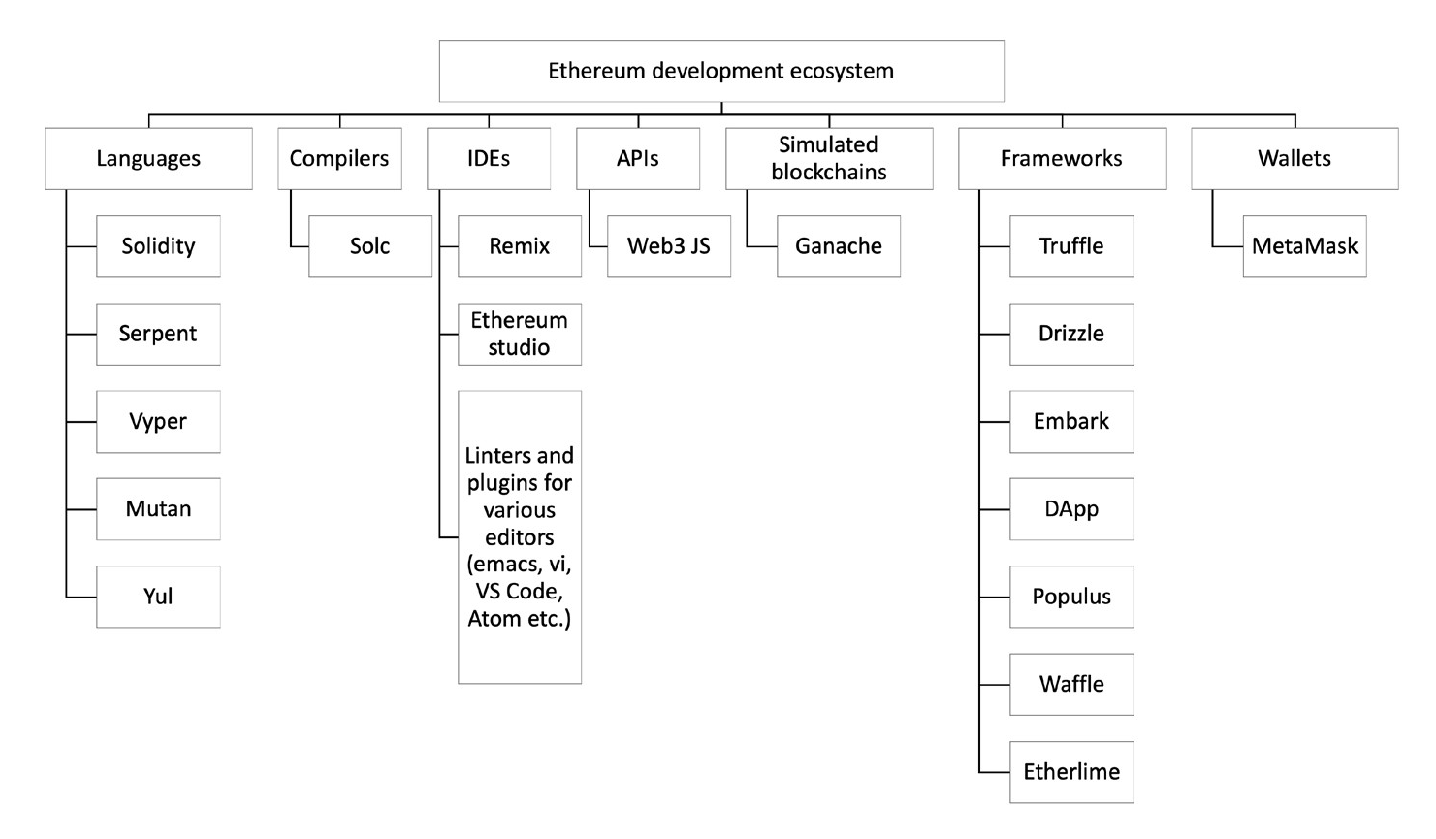
\includegraphics{figuras/taxonomia-componentes-de-desenvolvimento.pdf}
\end{frame}

\begin{frame}[fragile,allowframebreaks]{Linguagens}
\protect\hypertarget{linguagens}{}
\begin{itemize}
\tightlist
\item
  \textbf{Solidity:} Tem se tornado a linguagem padrão para escrever
  contratos para \emph{Ethereum}. O código precisa ser compilado e
  transformado em \emph{bytecode}, é necessário utilizar o compilador
  \texttt{solc}.
\item
  Vyper: This language is a Python-like experimental language that is
  being developed to bring security, simplicity, and auditability to
  smart contract development.
\item
  Yul: This is an intermediate language that has the ability to compile
  to different backends such as EVM and eWasm. The design goals of Yul
  mainly include readability, easy control flow, optimization, formal
  verification, and simplicity.
\item
  Mutan: This is a Go-style language, which was deprecated in early 2015
  and is no longer used.
\item
  LLL: This is a Low-Level Lisp-Like Language, hence the name LLL. This
  is also no longer used.
\item
  Serpent: This is a simple and clean Python-like language. It is not
  used for contract development anymore and is not supported by the
  community.
\item
  Leia mais sobre Solidity e Recursos de Desenvolvimento de
  \texttt{DApps} em
  \href{http://ethdocs.org/en/latest/contracts-and-transactions/developer-tools.html\#developer-tools}{DAPP
  DEVELOPMENT FRAMEWORKS\footnote<.->{\url{http://ethdocs.org/en/latest/contracts-and-transactions/developer-tools.html\#developer-tools}}}
\end{itemize}
\end{frame}

\begin{frame}[allowframebreaks]{Compiladores}
\protect\hypertarget{compiladores}{}
\begin{itemize}
\tightlist
\item
  The Solidity compiler (solc)
\item
  Compiler used to compile smart contract code and convert it into
  bytecode
\end{itemize}
\end{frame}

\begin{frame}[fragile,allowframebreaks]{Ferramentas e Bibliotecas}
\protect\hypertarget{ferramentas-e-bibliotecas}{}
\begin{itemize}
\tightlist
\item
  \texttt{Ganache}

  \begin{itemize}
  \tightlist
  \item
    Simula um Blockchain Ethereum pessoal com uma interface com usuário
    (UI), comumente usada no desenvolvimento e testes.
  \end{itemize}
\item
  \texttt{Ganache-cli}

  \begin{itemize}
  \tightlist
  \item
    Versão linha de comando do \texttt{Ganache} tem como pre-requisito
    \texttt{NodeJS}.
  \end{itemize}
\end{itemize}

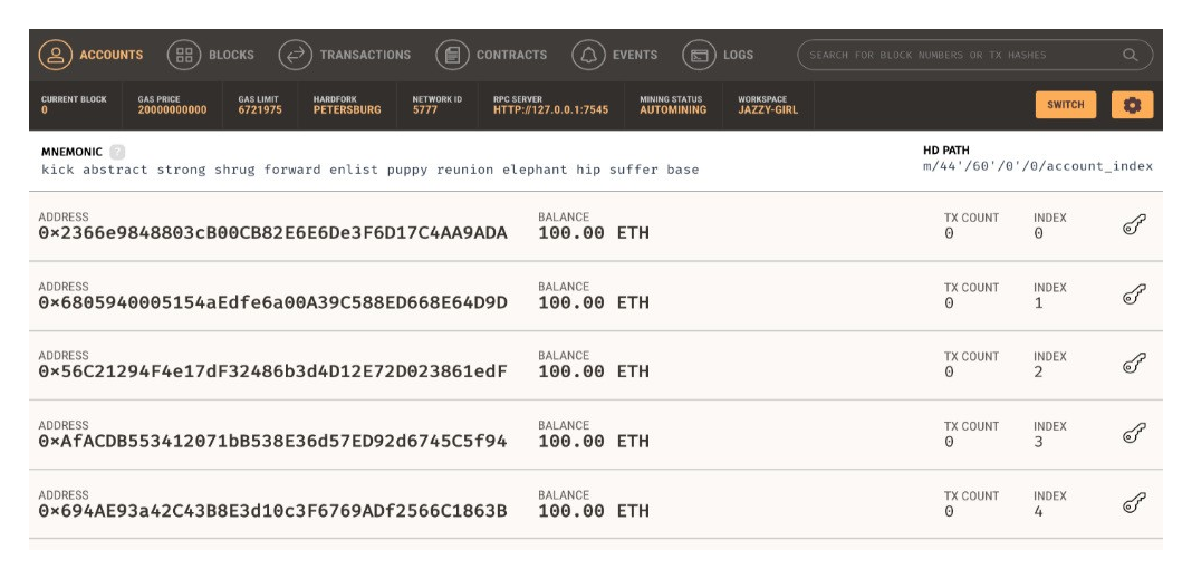
\includegraphics{figuras/ganache-interface.pdf}
\end{frame}

\begin{frame}[allowframebreaks]{Frameworks}
\protect\hypertarget{frameworks}{}
\begin{itemize}
\tightlist
\item
  \textbf{Truffle}

  \begin{itemize}
  \tightlist
  \item
    Framework de desenvolvimento para \emph{Ethereum} com recursos para
    implantação, teste e depuração.
  \end{itemize}
\end{itemize}

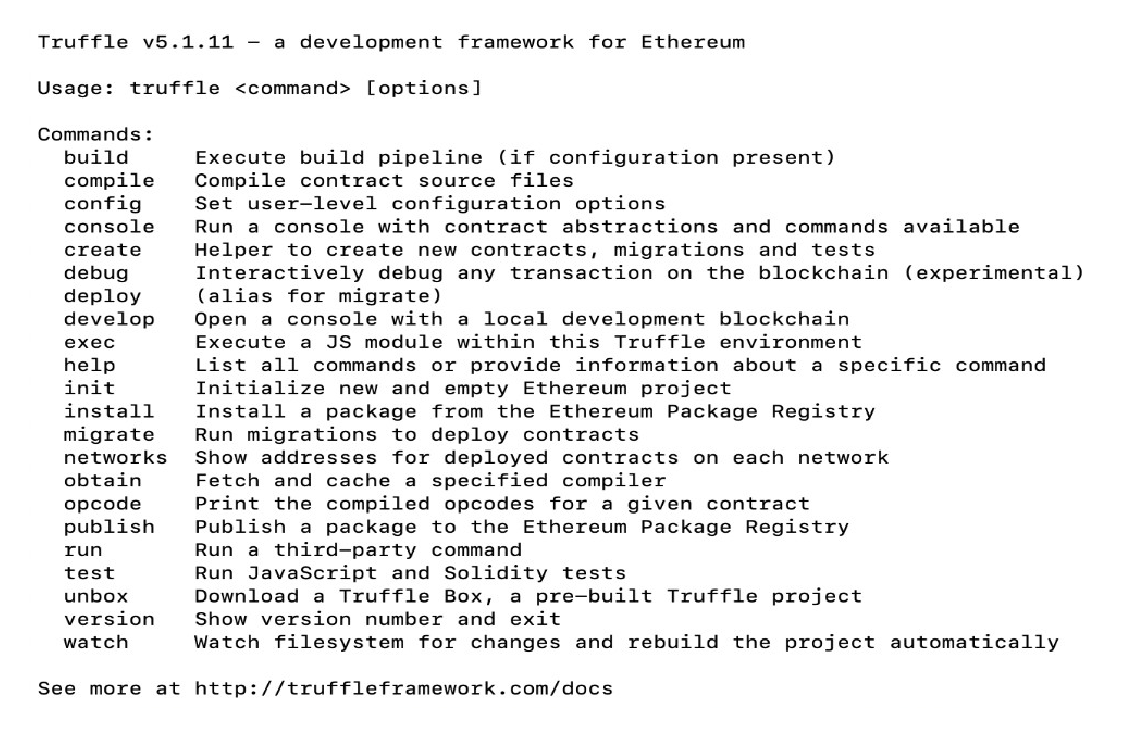
\includegraphics{figuras/truffle-interface.pdf}

\begin{itemize}
\tightlist
\item
  \textbf{Drizzle}

  \begin{itemize}
  \tightlist
  \item
    A set of frontend libraries for the development of web UIs
  \item
    Makes frontend development for DApps easie
  \item
    Requires NodeJS
  \item
    Based on the Redux store
  \item
    Maintains a library of React components
  \end{itemize}
\end{itemize}
\end{frame}

\begin{frame}[allowframebreaks]{Outras Ferramentas}
\protect\hypertarget{outras-ferramentas}{}
\begin{itemize}
\tightlist
\item
  Embark: powerful developer platform for building and deploying DApps
\item
  Brownie: framework for Ethereum smart contract development and testing
\item
  Waffle: another framework for smart contract development and testing
\item
  Etherlime: framework that allows DApp development, debugging, testing,
  and testing in Solidity and Vyper
\item
  OpenZeppelin: a toolkit for smart contract development
\end{itemize}
\end{frame}

\begin{frame}[allowframebreaks]{Contract development and deployment}
\protect\hypertarget{contract-development-and-deployment}{}
\begin{itemize}
\tightlist
\item
  Writing smart contracts is concerned with writing the contract source
  code in Solidity in a text editor.
\item
  There are various plugins and add-ons available for Vim in Linux,
  Atom, and other editors that provide syntax highlighting and
  formatting for Solidity source code.
\end{itemize}

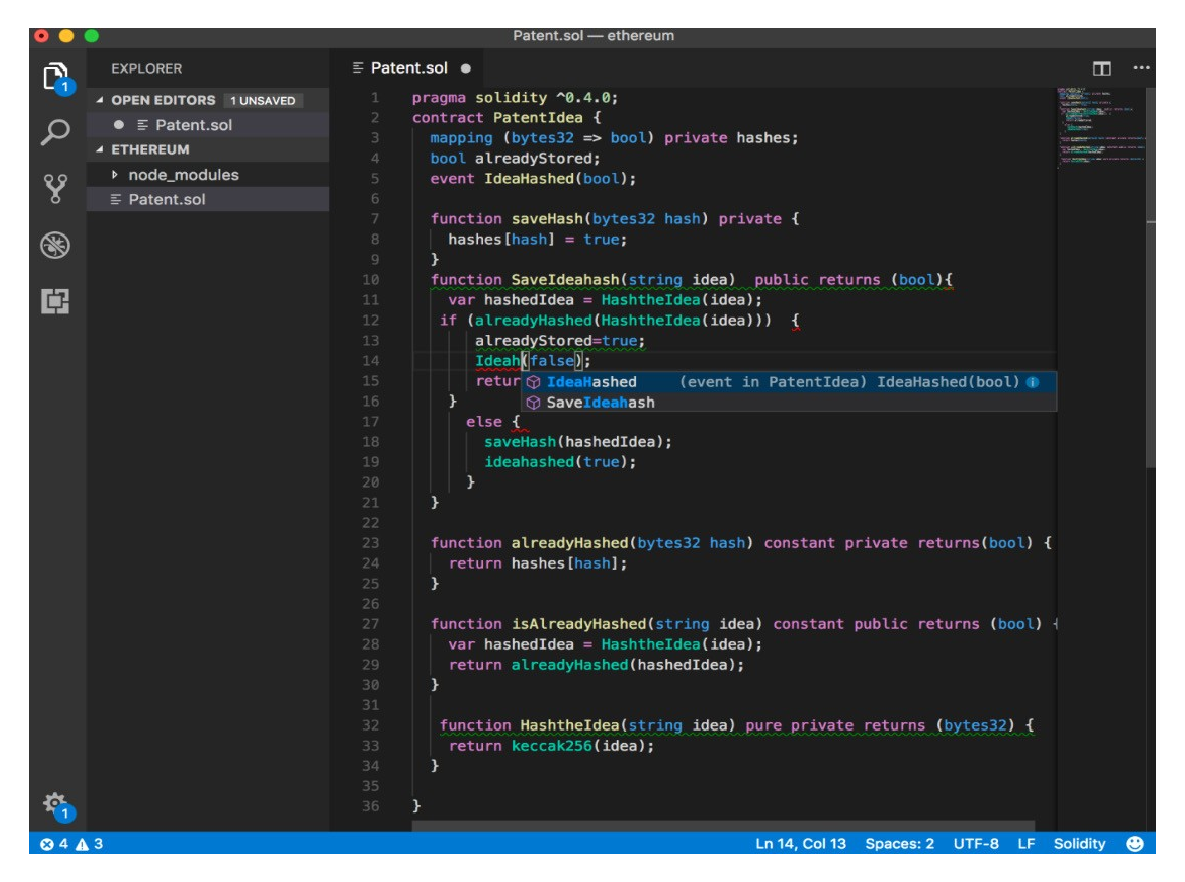
\includegraphics{figuras/vscode-interface.pdf}
\end{frame}

\begin{frame}[allowframebreaks]{The layout of a Solidity source code
file}
\protect\hypertarget{the-layout-of-a-solidity-source-code-file}{}
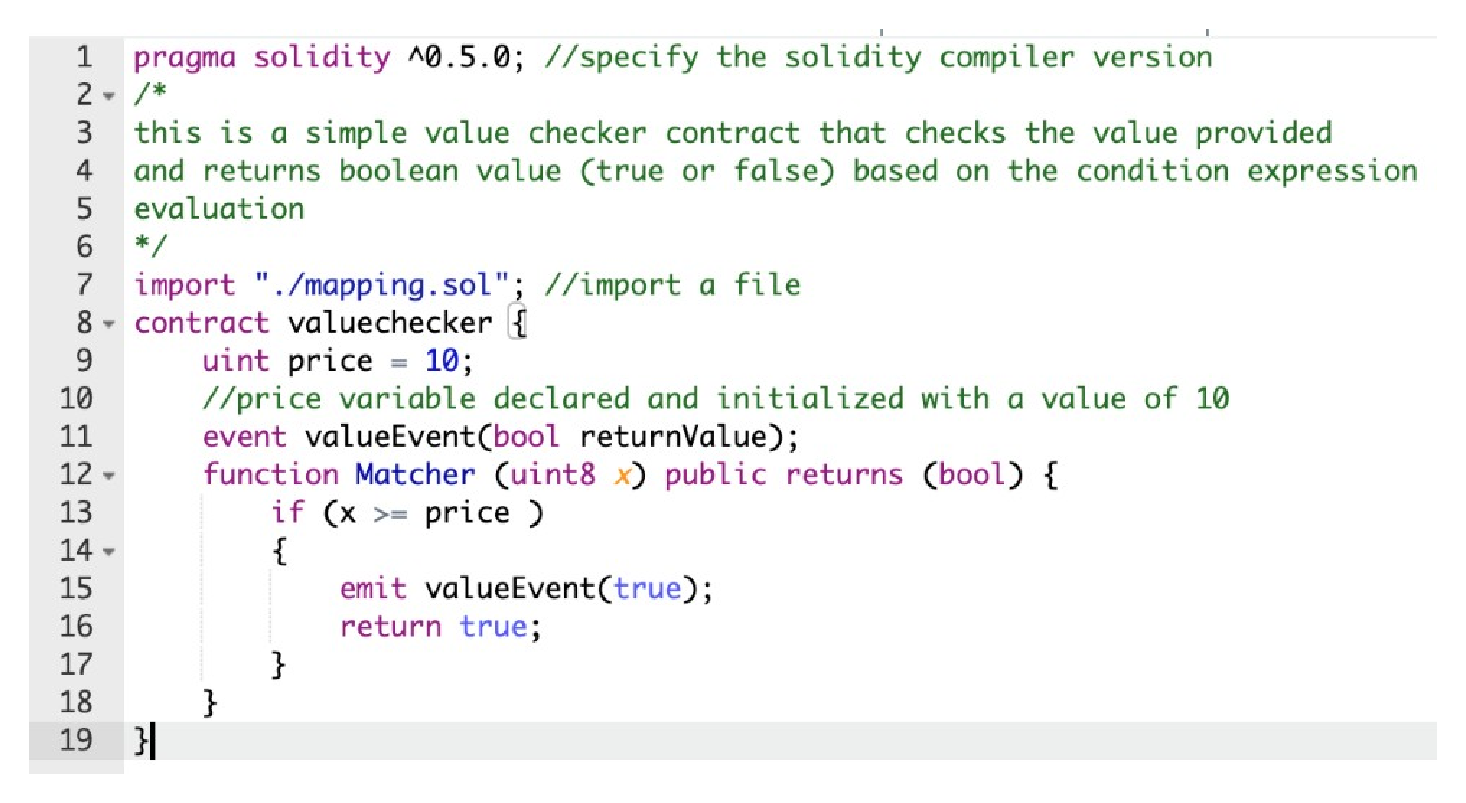
\includegraphics{figuras/solidity-example.pdf}
\end{frame}

\begin{frame}[allowframebreaks]{Linguagem Solidity}
\protect\hypertarget{linguagem-solidity}{}
\begin{itemize}
\tightlist
\item
  Uma Linguagem de Domínio Especiífico (DSL)
\item
  \emph{Contract-oriented language}
\item
  JavaScript / C-like
\item
  Amplamente utilizada
\item
  Estaticamente Tipada
\end{itemize}
\end{frame}

\begin{frame}[allowframebreaks]{Linguagem Solidity}
\protect\hypertarget{linguagem-solidity-1}{}
\end{frame}

\begin{frame}{Leitura Recomendada}
\protect\hypertarget{leitura-recomendada}{}
\normalsize

\begin{alertblock}{Leitura Recomendada}

\begin{alertblock}{Leitura Recomendada}

\textbf{Capítulo 14: Development Tools and Frameworks}

\textbf{Livro}:
\href{https://search.ebscohost.com/login.aspx?direct=true\&db=e000xww\&AN=1789486\&authtype=shib\&lang=pt-br\&site=eds-live\&scope=site\&ebv=EB\&ppid=pp_276}{IMRAN
BASHIR. Mastering Blockchain\,: Distributed Ledger Technology,
Decentralization, and Smart Contracts Explained, 2nd Edition.}

\end{alertblock}
\end{frame}

\hypertarget{pruxf3ximas-aulas}{%
\section{Próximas Aulas}\label{pruxf3ximas-aulas}}

\begin{frame}{Próximas Aulas}
\protect\hypertarget{pruxf3ximas-aulas-1}{}
\begin{itemize}
\tightlist
\item
  Ambientes de Desenvolvimento e Ferramentas.
\end{itemize}
\end{frame}

\hypertarget{referuxeancias}{%
\section{Referências}\label{referuxeancias}}

\begin{frame}[fragile,allowframebreaks]{Referências}
\protect\hypertarget{referuxeancias-1}{}
\normalsize

\hypertarget{refs}{}
\begin{CSLReferences}{1}{0}
\leavevmode\vadjust pre{\hypertarget{ref-178948620180101}{}}%
Imran, Bashir. 2018. \emph{Mastering Blockchain : Distributed Ledger
Technology, Decentralization, and Smart Contracts Explained, 2nd
Edition.} Packt Publishing.
\url{https://search.ebscohost.com/login.aspx?direct=true\&db=e000xww\&AN=1789486\&lang=pt-br\&site=eds-live\&scope=site}.

\end{CSLReferences}
\end{frame}

\end{document}
